\documentclass{standalone}

\usepackage{tikz}
\usepackage{standalone}
\usepackage{color}
\usetikzlibrary{calc}
\usepackage{pgfplots}

\begin{document}

    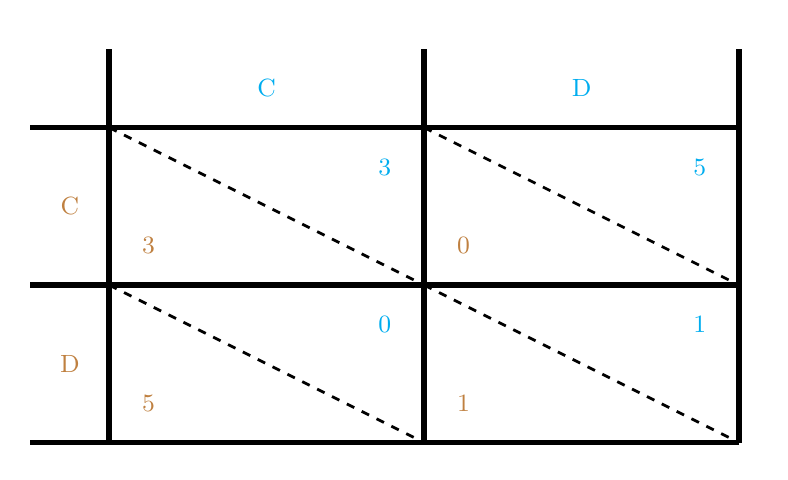
\begin{tikzpicture}
    \tikzstyle{state}=[minimum width=1cm, font=\boldmath];

    % horizontal lines
    \draw[-, line width=2pt] (-1, -2) -- (8, -2) node[right] {};
    \draw[-, line width=2pt] (-1, 0) -- (8, 0) node[right] {};
    \draw[-, line width=2pt] (-1, 2) -- (8, 2) node[right] {};

    % vertical lines
    \draw[-, line width=2pt] (0,-2) -- (0,3) node[above] {};
    \draw[-, line width=2pt] (4,-2) -- (4,3) node[above] {};
    \draw[-, line width=2pt] (8,-2) -- (8,3) node[above] {};

    % dashed lines
    \draw[dashed, line width=1pt] (0, 2) -- (4, 0) node[right] {};
    \draw[dashed, line width=1pt] (4, 2) -- (8, 0) node[right] {};
    \draw[dashed, line width=1pt] (0, 0) -- (4, -2) node[right] {};
    \draw[dashed, line width=1pt] (4, 0) -- (8, -2) node[right] {};

    % player's actions
    \node[circle, thick] (0) at (2, 2.5) [state] {\small \textcolor{cyan}C};
    \node[circle, thick] (0) at (6, 2.5) [state] {\small \textcolor{cyan}D};
    \node[circle, thick] (0) at (-0.5, 1) [state] {\small \textcolor{brown}C};
    \node[circle, thick] (0) at (-0.5, -1) [state] {\small \textcolor{brown}D};

    % payoffs
    \node[circle, thick] (0) at (3.5, 1.5) [state] {\small \textcolor{cyan}3};
    \node[circle, thick] (0) at (3.5, -0.5) [state] {\small \textcolor{cyan}0};
    \node[circle, thick] (0) at (0.5, 0.5) [state] {\small \textcolor{brown}3};
    \node[circle, thick] (0) at (0.5, -1.5) [state] {\small \textcolor{brown}5};
    \node[circle, thick] (0) at (7.5, 1.5) [state] {\small \textcolor{cyan}5};
    \node[circle, thick] (0) at (7.5, -0.5) [state] {\small \textcolor{cyan}1};
    \node[circle, thick] (0) at (4.5, 0.5) [state] {\small \textcolor{brown}0};
    \node[circle, thick] (0) at (4.5, -1.5) [state] {\small \textcolor{brown}1};

    \end{tikzpicture}

\end{document}